\subsection*{Validation run on Task 5}
Model behind every role: \texttt{claude-cli:claude-sonnet-5-5}. Turns: 6; orchestrator decisions: 3.

\textbf{Free-run error printed by the script that ran} (\texttt{silverbox\_pinn.py}): test RMSE $= 0.00100889$\,V, train RMSE $= 0.00144579$\,V.

\begin{longtable}{@{}r l p{0.72\linewidth}@{}}
\toprule \# & role & what it did\\ \midrule \endhead
1 & user & Please solve the following task with your team and report the verified free-run errors. Task 5. PINN (Physics Informed Neural Network) for the Silv...\\
2 & orchestrator & -\textgreater{} scientist: A plan must be written by the scientist before any code can be executed.\\
3 & scientist & \# Plan for Task 5: Silverbox PINN No numbers have been measured yet. Every size below is an expectation from the problem statement, not a result. \#...\\
4 & orchestrator & -\textgreater{} executor: The plan is complete, so it must now be coded and run to obtain verified RMSE values.\\
5 & executor & write silverbox\_pinn.py: ok run silverbox\_pinn.py: exit code 0, 210.0 s VERIFIED printed by the script: TEST\_RMSE=0.0010088887947707441, TRAIN\_RMSE=0.0014457...\\
6 & orchestrator & -\textgreater{} finish: A VERIFIED executor result with both TRAIN\_RMSE and TEST\_RMSE exists, so the run can be finished.\\
\bottomrule
\end{longtable}
\begin{figure}[H]\centering
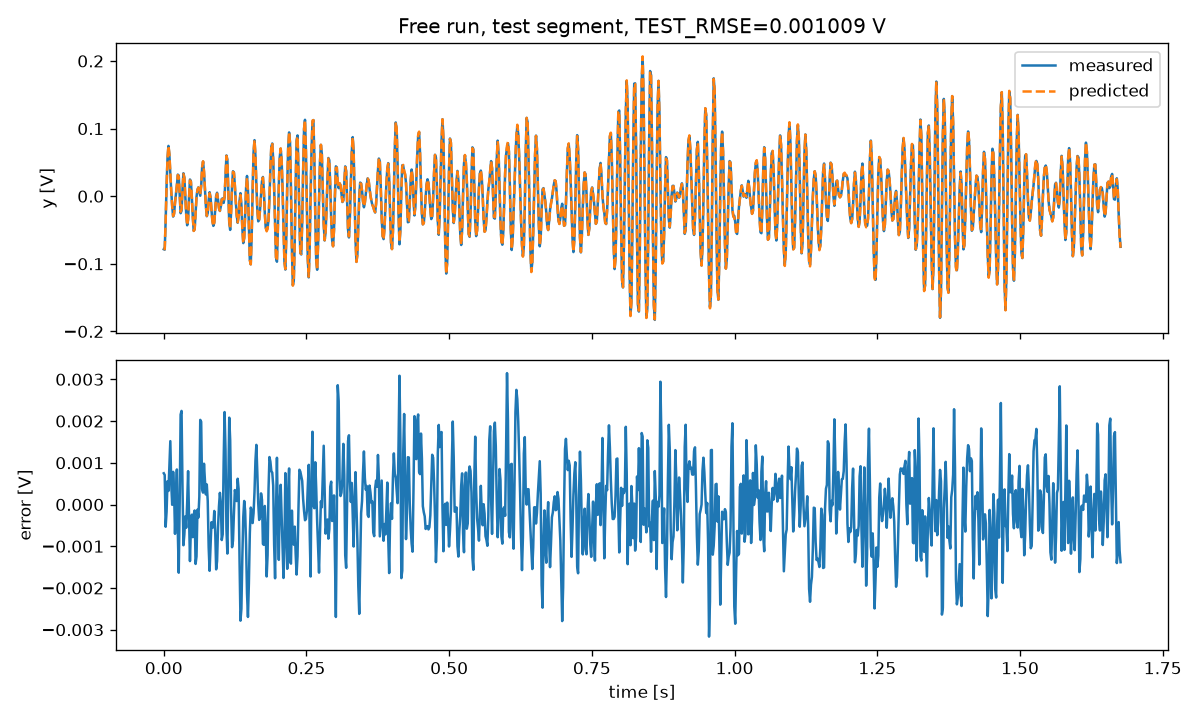
\includegraphics[width=0.85\linewidth]{../task6_agentic_system/runs/20261014-001143/work/test_segment.png}
\caption{The plot saved by the agents' script: measured output and free-run prediction on the test segment.}
\end{figure}

\paragraph{Transcript (abridged).}
\noindent\textbf{Turn 1 --- user}
\begin{lstlisting}
Please solve the following task with your team and report the verified free-run errors....
[the full Task 5 statement follows: task6_agentic_system/task5_statement.md]
\end{lstlisting}
\noindent\textbf{Turn 2 --- orchestrator}
\begin{lstlisting}
Decision 1/8 -> scientist
Instruction: Write the complete, code-ready plan for Task 5 (Silverbox PINN). Include: data loading from SNLS80mV.mat (V1=u, V2=y), slice [42650:46746], mean-centering, split 3072 train / 1024 test, dt=1/610.35. Network alpha_theta(y,v,u) with chosen depth/widths/activation and input/output scaling, optionally physics-informed initialization from eq. (1) (y''=-a v - b y - c y^3 + g u) with learnable a,b,c,g as a residual/prior (b ~ (2*pi*70)^2, a few tens). RK4 integration with u held/interpolated between samples (specify, e.g. midpoint u average), training scheme (multiple shooting over short windows, curriculum on window length, Adam then maybe LBFGS, learning rates, epochs), keeping total runtime under 5 minutes on CPU. Then the final free run: initial state from the first sample with finite-difference velocity, integrate through train into test without reading test y, print TRAIN_RMSE and TEST_RMSE, and save a plot of measured vs predicted on the test segment. Give a numbered list of steps specific enough to code.
Reason: A plan must be written by the scientist before any code can be executed.
\end{lstlisting}
\noindent\textbf{Turn 3 --- scientist}
\begin{lstlisting}
# Plan for Task 5: Silverbox PINN

No numbers have been measured yet. Every size below is an expectation from the problem statement, not a result.

## 1. Differential equation and coefficients

y'' + a y' + b y + c y^3 = g u(t), with y and u the mean-centered signals.

| Coef | Meaning | Expected size / initial value |
|---|---|---|
| a | damping, 1/s | tens, about 20-40 |
| b | linear stiffness, 1/s^2 | (2pi*70)^2 ~ 1.9e5 |
| c | cubic stiffness, 1/(V^2*s^2) | cy^2 ~ 0.1-0.3*b at |y| = 0.2, so c ~ 5e5-1.5e6 |
| g | input gain, V/(V*s^2) | order 1e4 (from y ~ g*u/(a*omega) at resonance); fix it by regression |

- a, b, c and g are four learnable scalars of the physics prior. They are not network weights.
- Initialize them by least squares on the training record (step 4), then refine them by shooting.
- The RK4 step at 70 Hz has omega*dt ~ 0.72, so the integrator carries phase and damping error of its own. Training and testing use the same integrator, so the fitted b and a will absorb this. This is intended and should not be "corrected".

## 2. Network

Acceleration: alpha_theta(y,v,u) = -a v - b y - c y^3 + g u + S_alpha * N_theta(y/S_y, v/S_v, u/S_u)

- **Scales** (computed from the training record only):
  - S_y = std(y_train)
  - S_v = omega?*S_y with omega? = 2pi*70
  - S_u = std(u_train)
  - S_alpha = omega?^2*S_y
- **MLP N_theta:** 3 -> 32 -> 32 -> 1, tanh activation, flo
[... abridged ...]
 after that run.

## Revision rules, if the first results are poor

- Keep eq. (1) and the free-run test unchanged.
- Diagnose from the train free-run error and the loss history, not from the test error.
- The first levers are a longer L in stage 3, 2 substeps per sample, a lower ?, and a larger network (64 units).
- If the rollout diverges, lower the learning rate and raise ?.
\end{lstlisting}
\noindent\textbf{Turn 4 --- orchestrator}
\begin{lstlisting}
Decision 2/8 -> executor
Instruction: Implement the scientist's latest plan (Silverbox PINN) in a new Python file and run it (5-minute limit). Follow the numbered steps exactly: load SNLS80mV.mat, slice [42650:46746], center, 3072/1024 split, least-squares init of a,b,c,g, physics-prior + zero-init residual MLP (3-32-32-1 tanh, float64), RK4 with midpoint u, multiple-shooting stages 0-3 (optional 4) with wall-clock guards, then one free run from sample 0 through train into test reading only u. Save the plot of measured vs predicted on the test segment to test_segment.png. Print the final a,b,c,g, and as the last two lines TRAIN_RMSE=<float> and TEST_RMSE=<float>. Return the printed output verbatim, or the full traceback if it fails.
Reason: The plan is complete, so it must now be coded and run to obtain verified RMSE values.
\end{lstlisting}
\noindent\textbf{Turn 5 --- executor}
\begin{lstlisting}
File: silverbox_pinn.py. Exit code: 0. Runtime was 207.6 s, inside the 5-minute limit. The plot was saved as test_segment.png.

Printed RMSE lines, exactly as printed:
TRAIN_RMSE=0.0014457934186479073
TEST_RMSE=0.0010088887947707441

Other printed values:
- Least-squares init: a=39.6, b=1.760e5, c=5.749e5, g=1.600e5.
- Final fitted values: a=41.19, b=1.848e5, c=7.4768e5, g=1.9608e5.
- Maximum |?| of the free run was 0.2068.
- The zero-predictor test RMSE was 0.0605.
- Training stage S3 hit its time budget at iteration 109 of 150.
- Stage 4 stopped after 8 iterations, at the 30 s budget.
- stderr held only a harmless PyTorch UserWarning about converting a tensor that requires grad to a float.

The free run started at sample 0 and carried its state through the train/test boundary. It read only u after the first sample.

[tool record]
write silverbox_pinn.py: ok
run silverbox_pinn.py: exit code 0, 210.0 s
VERIFIED printed by the script: TEST_RMSE=0.0010088887947707441, TRAIN_RMSE=0.0014457934186479073
\end{lstlisting}
\noindent\textbf{Turn 6 --- orchestrator}
\begin{lstlisting}
Decision 3/8 -> finish
Instruction: The Silverbox PINN ran and the script printed the free-run errors. The script is silverbox_pinn.py and the plot is test_segment.png.

Verified results, exactly as printed:
- TRAIN_RMSE=0.0014457934186479073
- TEST_RMSE=0.0010088887947707441

For scale, predicting zero scores 0.0605 V RMSE on the test segment, so the model is much better than the baseline.

Method:
- The model is eq. (1) as a physics prior with learnable a, b, c and g, plus a residual 3-32-32-1 tanh network whose last layer starts at zero.
- It was integrated with RK4 and trained by multiple shooting.
- The free run started at sample 0 with a finite-difference velocity. It carried the state through the train/test boundary and read only u after the first sample.

Fitted coefficients:
- Least-squares initialization: a=39.6, b=1.760e5, c=5.749e5, g=1.600e5.
- Final: a=41.19, b=1.848e5, c=7.4768e5, g=1.9608e5.

Other notes:
- The maximum |?| of the free run was 0.2068.
- The run took about 208 s.
- The last stage-3 and stage-4 runs stopped at their time budgets (iteration 109 of 150 and 8 iterations).
- stderr held only a harmless PyTorch UserWarning.
Reason: A VERIFIED executor result with both TRAIN_RMSE and TEST_RMSE exists, so the run can be finished.
\end{lstlisting}
